\documentclass[11pt]{article}

    \usepackage[breakable]{tcolorbox}
    \usepackage{parskip} % Stop auto-indenting (to mimic markdown behaviour)
    

    % Basic figure setup, for now with no caption control since it's done
    % automatically by Pandoc (which extracts !(path) syntax from Markdown).
    \usepackage{graphicx}
    % Maintain compatibility with old templates. Remove in nbconvert 6.0
    \let\Oldincludegraphics\includegraphics
    % Ensure that by default, figures have no caption (until we provide a
    % proper Figure object with a Caption API and a way to capture that
    % in the conversion process - todo).
    \usepackage{caption}
    \DeclareCaptionFormat{nocaption}{}
    \captionsetup{format=nocaption,aboveskip=0pt,belowskip=0pt}

    \usepackage{float}
    \floatplacement{figure}{H} % forces figures to be placed at the correct location
    \usepackage{xcolor} % Allow colors to be defined
    \usepackage{enumerate} % Needed for markdown enumerations to work
    \usepackage{geometry} % Used to adjust the document margins
    \usepackage{amsmath} % Equations
    \usepackage{amssymb} % Equations
    \usepackage{textcomp} % defines textquotesingle
    % Hack from http://tex.stackexchange.com/a/47451/13684:
    \AtBeginDocument{%
        \def\PYZsq{\textquotesingle}% Upright quotes in Pygmentized code
    }
    \usepackage{upquote} % Upright quotes for verbatim code
    \usepackage{eurosym} % defines \euro

    \usepackage{iftex}
\ifPDFTeX
    \usepackage[T1]{fontenc}
    \usepackage[utf8]{inputenc}
\else
    \usepackage{fontspec}
    \usepackage{unicode-math}
\fi


    \usepackage{listings}
    \lstset{basicstyle=\ttfamily\small,breaklines=true}

    \usepackage{fancyvrb} % verbatim replacement that allows latex
    \usepackage{grffile} % extends the file name processing of package graphics
                         % to support a larger range
    \makeatletter % fix for old versions of grffile with XeLaTeX
    \@ifpackagelater{grffile}{2019/11/01}
    {
      % Do nothing on new versions
    }
    {
      \def\Gread@@xetex#1{%
        \IfFileExists{"\Gin@base".bb}%
        {\Gread@eps{\Gin@base.bb}}%
        {\Gread@@xetex@aux#1}%
      }
    }
    \makeatother
    \usepackage[Export]{adjustbox} % Used to constrain images to a maximum size
    \adjustboxset{max size={0.9\linewidth}{0.9\paperheight}}

    % The hyperref package gives us a pdf with properly built
    % internal navigation ('pdf bookmarks' for the table of contents,
    % internal cross-reference links, web links for URLs, etc.)
    \usepackage{hyperref}
    % The default LaTeX title has an obnoxious amount of whitespace. By default,
    % titling removes some of it. It also provides customization options.
    \usepackage{titling}
    \usepackage{longtable} % longtable support required by pandoc >1.10
    \usepackage{booktabs}  % table support for pandoc > 1.12.2
    \usepackage{array}     % table support for pandoc >= 2.11.3
    \usepackage{calc}      % table minipage width calculation for pandoc >= 2.11.1
    \usepackage[inline]{enumitem} % IRkernel/repr support (it uses the enumerate* environment)
    %\usepackage[normalem]{ulem} % ulem is needed to support strikethroughs (\sout)
                                % normalem makes italics be italics, not underlines
    \usepackage{mathrsfs}
    \usepackage{tikz}
    \usetikzlibrary{arrows.meta,positioning}
    

    
    % Colors for the hyperref package
    \definecolor{urlcolor}{rgb}{0,.145,.698}
    \definecolor{linkcolor}{rgb}{.71,0.21,0.01}
    \definecolor{citecolor}{rgb}{.12,.54,.11}

    % ANSI colors
    \definecolor{ansi-black}{HTML}{3E424D}
    \definecolor{ansi-black-intense}{HTML}{282C36}
    \definecolor{ansi-red}{HTML}{E75C58}
    \definecolor{ansi-red-intense}{HTML}{B22B31}
    \definecolor{ansi-green}{HTML}{00A250}
    \definecolor{ansi-green-intense}{HTML}{007427}
    \definecolor{ansi-yellow}{HTML}{DDB62B}
    \definecolor{ansi-yellow-intense}{HTML}{B27D12}
    \definecolor{ansi-blue}{HTML}{208FFB}
    \definecolor{ansi-blue-intense}{HTML}{0065CA}
    \definecolor{ansi-magenta}{HTML}{D160C4}
    \definecolor{ansi-magenta-intense}{HTML}{A03196}
    \definecolor{ansi-cyan}{HTML}{60C6C8}
    \definecolor{ansi-cyan-intense}{HTML}{258F8F}
    \definecolor{ansi-white}{HTML}{C5C1B4}
    \definecolor{ansi-white-intense}{HTML}{A1A6B2}
    \definecolor{ansi-default-inverse-fg}{HTML}{FFFFFF}
    \definecolor{ansi-default-inverse-bg}{HTML}{000000}

    % common color for the border for error outputs.
    \definecolor{outerrorbackground}{HTML}{FFDFDF}

    % commands and environments needed by pandoc snippets
    % extracted from the output of `pandoc -s`
    \providecommand{}{%
      \setlength{\bibitem{gross}sep}{0pt}\setlength{\parskip}{0pt}}
    \DefineVerbatimEnvironment{Highlighting}{Verbatim}{commandchars=\\\{\}}
    % Add ',fontsize=\small' for more characters per line
\newenvironment{Shaded}{}{}
\newcommand{\KeywordTok}[1]{\textcolor[rgb]{0.00,0.44,0.13}{\textbf{{#1}}}}
\newcommand{\DataTypeTok}[1]{\textcolor[rgb]{0.56,0.13,0.00}{{#1}}}
\newcommand{\DecValTok}[1]{\textcolor[rgb]{0.25,0.63,0.44}{{#1}}}
\newcommand{\BaseNTok}[1]{\textcolor[rgb]{0.25,0.63,0.44}{{#1}}}
\newcommand{\FloatTok}[1]{\textcolor[rgb]{0.25,0.63,0.44}{{#1}}}
\newcommand{\CharTok}[1]{\textcolor[rgb]{0.25,0.44,0.63}{{#1}}}
\newcommand{\StringTok}[1]{\textcolor[rgb]{0.25,0.44,0.63}{{#1}}}
\newcommand{\CommentTok}[1]{\textcolor[rgb]{0.38,0.63,0.69}{\textit{{#1}}}}
\newcommand{\OtherTok}[1]{\textcolor[rgb]{0.00,0.44,0.13}{{#1}}}
\newcommand{\AlertTok}[1]{\textcolor[rgb]{1.00,0.00,0.00}{\textbf{{#1}}}}
\newcommand{\FunctionTok}[1]{\textcolor[rgb]{0.02,0.16,0.49}{{#1}}}
\newcommand{\RegionMarkerTok}[1]{{#1}}
\newcommand{\ErrorTok}[1]{\textcolor[rgb]{1.00,0.00,0.00}{\textbf{{#1}}}}
\newcommand{\NormalTok}[1]{{#1}}

    % Additional commands for more recent versions of Pandoc
\newcommand{\ConstantTok}[1]{\textcolor[rgb]{0.53,0.00,0.00}{{#1}}}
\newcommand{\SpecialCharTok}[1]{\textcolor[rgb]{0.25,0.44,0.63}{{#1}}}
\newcommand{\VerbatimStringTok}[1]{\textcolor[rgb]{0.25,0.44,0.63}{{#1}}}
\newcommand{\SpecialStringTok}[1]{\textcolor[rgb]{0.73,0.40,0.53}{{#1}}}
\newcommand{\ImportTok}[1]{{#1}}
\newcommand{\DocumentationTok}[1]{\textcolor[rgb]{0.73,0.13,0.13}{\textit{{#1}}}}
\newcommand{\AnnotationTok}[1]{\textcolor[rgb]{0.38,0.63,0.69}{\textbf{\textit{{#1}}}}}
\newcommand{\CommentVarTok}[1]{\textcolor[rgb]{0.38,0.63,0.69}{\textbf{\textit{{#1}}}}}
\newcommand{\VariableTok}[1]{\textcolor[rgb]{0.10,0.09,0.49}{{#1}}}
\newcommand{\ControlFlowTok}[1]{\textcolor[rgb]{0.00,0.44,0.13}{\textbf{{#1}}}}
\newcommand{\OperatorTok}[1]{\textcolor[rgb]{0.40,0.40,0.40}{{#1}}}
\newcommand{\BuiltInTok}[1]{{#1}}
\newcommand{\ExtensionTok}[1]{{#1}}
\newcommand{\PreprocessorTok}[1]{\textcolor[rgb]{0.74,0.48,0.00}{{#1}}}
\newcommand{\AttributeTok}[1]{\textcolor[rgb]{0.49,0.56,0.16}{{#1}}}
\newcommand{\InformationTok}[1]{\textcolor[rgb]{0.38,0.63,0.69}{\textbf{\textit{{#1}}}}}
\newcommand{\WarningTok}[1]{\textcolor[rgb]{0.38,0.63,0.69}{\textbf{\textit{{#1}}}}}


    % Define a nice break command that doesn't care if a line doesn't already
    % exist.
    \def\br{\hspace*{\fill} \\* }
    % Math Jax compatibility definitions
    \def\gt{>}
    \def\lt{<}
    \let\Oldtex\TeX
    \let\Oldlatex\LaTeX
    \renewcommand{\TeX}{\textrm{\Oldtex}}
    \renewcommand{\LaTeX}{\textrm{\Oldlatex}}
    % Document parameters
    % Document title
    \title{informe\_matematico}
    
    
    
    
    
    
    
% Pygments definitions
\makeatletter
\def\PY@reset{\let\PY@it=\relax \let\PY@bf=\relax%
    \let\PY@ul=\relax \let\PY@tc=\relax%
    \let\PY@bc=\relax \let\PY@ff=\relax}
\def\PY@tok#1{\csname PY@tok@#1\endcsname}
\def\PY@toks#1+{\ifx\relax#1\empty\else%
    \PY@tok{#1}\expandafter\PY@toks\fi}
\def\PY@do#1{\PY@bc{\PY@tc{\PY@ul{%
    \PY@it{\PY@bf{\PY@ff{#1}}}}}}}
\def\PY#1#2{\PY@reset\PY@toks#1+\relax+\PY@do{#2}}

\@namedef{PY@tok@w}{\def\PY@tc##1{\textcolor[rgb]{0.73,0.73,0.73}{##1}}}
\@namedef{PY@tok@c}{\let\PY@it=\textit\def\PY@tc##1{\textcolor[rgb]{0.24,0.48,0.48}{##1}}}
\@namedef{PY@tok@cp}{\def\PY@tc##1{\textcolor[rgb]{0.61,0.40,0.00}{##1}}}
\@namedef{PY@tok@k}{\let\PY@bf=\textbf\def\PY@tc##1{\textcolor[rgb]{0.00,0.50,0.00}{##1}}}
\@namedef{PY@tok@kp}{\def\PY@tc##1{\textcolor[rgb]{0.00,0.50,0.00}{##1}}}
\@namedef{PY@tok@kt}{\def\PY@tc##1{\textcolor[rgb]{0.69,0.00,0.25}{##1}}}
\@namedef{PY@tok@o}{\def\PY@tc##1{\textcolor[rgb]{0.40,0.40,0.40}{##1}}}
\@namedef{PY@tok@ow}{\let\PY@bf=\textbf\def\PY@tc##1{\textcolor[rgb]{0.67,0.13,1.00}{##1}}}
\@namedef{PY@tok@nb}{\def\PY@tc##1{\textcolor[rgb]{0.00,0.50,0.00}{##1}}}
\@namedef{PY@tok@nf}{\def\PY@tc##1{\textcolor[rgb]{0.00,0.00,1.00}{##1}}}
\@namedef{PY@tok@nc}{\let\PY@bf=\textbf\def\PY@tc##1{\textcolor[rgb]{0.00,0.00,1.00}{##1}}}
\@namedef{PY@tok@nn}{\let\PY@bf=\textbf\def\PY@tc##1{\textcolor[rgb]{0.00,0.00,1.00}{##1}}}
\@namedef{PY@tok@ne}{\let\PY@bf=\textbf\def\PY@tc##1{\textcolor[rgb]{0.80,0.25,0.22}{##1}}}
\@namedef{PY@tok@nv}{\def\PY@tc##1{\textcolor[rgb]{0.10,0.09,0.49}{##1}}}
\@namedef{PY@tok@no}{\def\PY@tc##1{\textcolor[rgb]{0.53,0.00,0.00}{##1}}}
\@namedef{PY@tok@nl}{\def\PY@tc##1{\textcolor[rgb]{0.46,0.46,0.00}{##1}}}
\@namedef{PY@tok@ni}{\let\PY@bf=\textbf\def\PY@tc##1{\textcolor[rgb]{0.44,0.44,0.44}{##1}}}
\@namedef{PY@tok@na}{\def\PY@tc##1{\textcolor[rgb]{0.41,0.47,0.13}{##1}}}
\@namedef{PY@tok@nt}{\let\PY@bf=\textbf\def\PY@tc##1{\textcolor[rgb]{0.00,0.50,0.00}{##1}}}
\@namedef{PY@tok@nd}{\def\PY@tc##1{\textcolor[rgb]{0.67,0.13,1.00}{##1}}}
\@namedef{PY@tok@s}{\def\PY@tc##1{\textcolor[rgb]{0.73,0.13,0.13}{##1}}}
\@namedef{PY@tok@sd}{\let\PY@it=\textit\def\PY@tc##1{\textcolor[rgb]{0.73,0.13,0.13}{##1}}}
\@namedef{PY@tok@si}{\let\PY@bf=\textbf\def\PY@tc##1{\textcolor[rgb]{0.64,0.35,0.47}{##1}}}
\@namedef{PY@tok@se}{\let\PY@bf=\textbf\def\PY@tc##1{\textcolor[rgb]{0.67,0.36,0.12}{##1}}}
\@namedef{PY@tok@sr}{\def\PY@tc##1{\textcolor[rgb]{0.64,0.35,0.47}{##1}}}
\@namedef{PY@tok@ss}{\def\PY@tc##1{\textcolor[rgb]{0.10,0.09,0.49}{##1}}}
\@namedef{PY@tok@sx}{\def\PY@tc##1{\textcolor[rgb]{0.00,0.50,0.00}{##1}}}
\@namedef{PY@tok@m}{\def\PY@tc##1{\textcolor[rgb]{0.40,0.40,0.40}{##1}}}
\@namedef{PY@tok@gh}{\let\PY@bf=\textbf\def\PY@tc##1{\textcolor[rgb]{0.00,0.00,0.50}{##1}}}
\@namedef{PY@tok@gu}{\let\PY@bf=\textbf\def\PY@tc##1{\textcolor[rgb]{0.50,0.00,0.50}{##1}}}
\@namedef{PY@tok@gd}{\def\PY@tc##1{\textcolor[rgb]{0.63,0.00,0.00}{##1}}}
\@namedef{PY@tok@gi}{\def\PY@tc##1{\textcolor[rgb]{0.00,0.52,0.00}{##1}}}
\@namedef{PY@tok@gr}{\def\PY@tc##1{\textcolor[rgb]{0.89,0.00,0.00}{##1}}}
\@namedef{PY@tok@ge}{\let\PY@it=\textit}
\@namedef{PY@tok@gs}{\let\PY@bf=\textbf}
\@namedef{PY@tok@ges}{\let\PY@bf=\textbf\let\PY@it=\textit}
\@namedef{PY@tok@gp}{\let\PY@bf=\textbf\def\PY@tc##1{\textcolor[rgb]{0.00,0.00,0.50}{##1}}}
\@namedef{PY@tok@go}{\def\PY@tc##1{\textcolor[rgb]{0.44,0.44,0.44}{##1}}}
\@namedef{PY@tok@gt}{\def\PY@tc##1{\textcolor[rgb]{0.00,0.27,0.87}{##1}}}
\@namedef{PY@tok@err}{\def\PY@bc##1{{\setlength{\fboxsep}{\string -\fboxrule}\fcolorbox[rgb]{1.00,0.00,0.00}{1,1,1}{\strut ##1}}}}
\@namedef{PY@tok@kc}{\let\PY@bf=\textbf\def\PY@tc##1{\textcolor[rgb]{0.00,0.50,0.00}{##1}}}
\@namedef{PY@tok@kd}{\let\PY@bf=\textbf\def\PY@tc##1{\textcolor[rgb]{0.00,0.50,0.00}{##1}}}
\@namedef{PY@tok@kn}{\let\PY@bf=\textbf\def\PY@tc##1{\textcolor[rgb]{0.00,0.50,0.00}{##1}}}
\@namedef{PY@tok@kr}{\let\PY@bf=\textbf\def\PY@tc##1{\textcolor[rgb]{0.00,0.50,0.00}{##1}}}
\@namedef{PY@tok@bp}{\def\PY@tc##1{\textcolor[rgb]{0.00,0.50,0.00}{##1}}}
\@namedef{PY@tok@fm}{\def\PY@tc##1{\textcolor[rgb]{0.00,0.00,1.00}{##1}}}
\@namedef{PY@tok@vc}{\def\PY@tc##1{\textcolor[rgb]{0.10,0.09,0.49}{##1}}}
\@namedef{PY@tok@vg}{\def\PY@tc##1{\textcolor[rgb]{0.10,0.09,0.49}{##1}}}
\@namedef{PY@tok@vi}{\def\PY@tc##1{\textcolor[rgb]{0.10,0.09,0.49}{##1}}}
\@namedef{PY@tok@vm}{\def\PY@tc##1{\textcolor[rgb]{0.10,0.09,0.49}{##1}}}
\@namedef{PY@tok@sa}{\def\PY@tc##1{\textcolor[rgb]{0.73,0.13,0.13}{##1}}}
\@namedef{PY@tok@sb}{\def\PY@tc##1{\textcolor[rgb]{0.73,0.13,0.13}{##1}}}
\@namedef{PY@tok@sc}{\def\PY@tc##1{\textcolor[rgb]{0.73,0.13,0.13}{##1}}}
\@namedef{PY@tok@dl}{\def\PY@tc##1{\textcolor[rgb]{0.73,0.13,0.13}{##1}}}
\@namedef{PY@tok@s2}{\def\PY@tc##1{\textcolor[rgb]{0.73,0.13,0.13}{##1}}}
\@namedef{PY@tok@sh}{\def\PY@tc##1{\textcolor[rgb]{0.73,0.13,0.13}{##1}}}
\@namedef{PY@tok@s1}{\def\PY@tc##1{\textcolor[rgb]{0.73,0.13,0.13}{##1}}}
\@namedef{PY@tok@mb}{\def\PY@tc##1{\textcolor[rgb]{0.40,0.40,0.40}{##1}}}
\@namedef{PY@tok@mf}{\def\PY@tc##1{\textcolor[rgb]{0.40,0.40,0.40}{##1}}}
\@namedef{PY@tok@mh}{\def\PY@tc##1{\textcolor[rgb]{0.40,0.40,0.40}{##1}}}
\@namedef{PY@tok@mi}{\def\PY@tc##1{\textcolor[rgb]{0.40,0.40,0.40}{##1}}}
\@namedef{PY@tok@il}{\def\PY@tc##1{\textcolor[rgb]{0.40,0.40,0.40}{##1}}}
\@namedef{PY@tok@mo}{\def\PY@tc##1{\textcolor[rgb]{0.40,0.40,0.40}{##1}}}
\@namedef{PY@tok@ch}{\let\PY@it=\textit\def\PY@tc##1{\textcolor[rgb]{0.24,0.48,0.48}{##1}}}
\@namedef{PY@tok@cm}{\let\PY@it=\textit\def\PY@tc##1{\textcolor[rgb]{0.24,0.48,0.48}{##1}}}
\@namedef{PY@tok@cpf}{\let\PY@it=\textit\def\PY@tc##1{\textcolor[rgb]{0.24,0.48,0.48}{##1}}}
\@namedef{PY@tok@c1}{\let\PY@it=\textit\def\PY@tc##1{\textcolor[rgb]{0.24,0.48,0.48}{##1}}}
\@namedef{PY@tok@cs}{\let\PY@it=\textit\def\PY@tc##1{\textcolor[rgb]{0.24,0.48,0.48}{##1}}}

\def\PYZbs{\char`\\}
\def\PYZus{\char`\_}
\def\PYZob{\char`\{}
\def\PYZcb{\char`\}}
\def\PYZca{\char`\^}
\def\PYZam{\char`\&}
\def\PYZlt{\char`\<}
\def\PYZgt{\char`\>}
\def\PYZsh{\char`\#}
\def\PYZpc{\char`\%}
\def\PYZdl{\char`\$}
\def\PYZhy{\char`\-}
\def\PYZsq{\char`\'}
\def\PYZdq{\char`\"}
\def\PYZti{\char`\~}
% for compatibility with earlier versions
\def\PYZat{@}
\def\PYZlb{[}
\def\PYZrb{]}
\makeatother


    % For linebreaks inside Verbatim environment from package fancyvrb.
    \makeatletter
\newbox\Wrappedcontinuationbox
\newbox\Wrappedvisiblespacebox
\newcommand*\Wrappedvisiblespace {\textcolor{red}{\textvisiblespace}}
\newcommand*\Wrappedcontinuationsymbol {\textcolor{red}{\llap{\tiny$\m@th\hookrightarrow$}}}
\newcommand*\Wrappedcontinuationindent {3ex }
\newcommand*\Wrappedafterbreak {\kern\Wrappedcontinuationindent\copy\Wrappedcontinuationbox}
        % Take advantage of the already applied Pygments mark-up to insert
        % potential linebreaks for TeX processing.
        %        {, <, #, %, $, ' and ": go to next line.
        %        _, }, ^, &, >, - and ~: stay at end of broken line.
        % Use of \textquotesingle for straight quote.
\newcommand*\Wrappedbreaksatspecials {%
            \def\PYGZus{\discretionary{\char`\_}{\Wrappedafterbreak}{\char`\_}}%
            \def\PYGZob{\discretionary{}{\Wrappedafterbreak\char`\{}{\char`\{}}%
            \def\PYGZcb{\discretionary{\char`\}}{\Wrappedafterbreak}{\char`\}}}%
            \def\PYGZca{\discretionary{\char`\^}{\Wrappedafterbreak}{\char`\^}}%
            \def\PYGZam{\discretionary{\char`\&}{\Wrappedafterbreak}{\char`\&}}%
            \def\PYGZlt{\discretionary{}{\Wrappedafterbreak\char`\<}{\char`\<}}%
            \def\PYGZgt{\discretionary{\char`\>}{\Wrappedafterbreak}{\char`\>}}%
            \def\PYGZsh{\discretionary{}{\Wrappedafterbreak\char`\#}{\char`\#}}%
            \def\PYGZpc{\discretionary{}{\Wrappedafterbreak\char`\%}{\char`\%}}%
            \def\PYGZdl{\discretionary{}{\Wrappedafterbreak\char`\$}{\char`\$}}%
            \def\PYGZhy{\discretionary{\char`\-}{\Wrappedafterbreak}{\char`\-}}%
            \def\PYGZsq{\discretionary{}{\Wrappedafterbreak\textquotesingle}{\textquotesingle}}%
            \def\PYGZdq{\discretionary{}{\Wrappedafterbreak\char`\"}{\char`\"}}%
            \def\PYGZti{\discretionary{\char`\~}{\Wrappedafterbreak}{\char`\~}}%
        }
        % Some characters . , ; ? ! / are not pygmentized.
        % This macro makes them "active" and they will insert potential linebreaks
\newcommand*\Wrappedbreaksatpunct {%
            \lccode`\~`\.\lowercase{\def~}{\discretionary{\hbox{\char`\.}}{\Wrappedafterbreak}{\hbox{\char`\.}}}%
            \lccode`\~`\,\lowercase{\def~}{\discretionary{\hbox{\char`\,}}{\Wrappedafterbreak}{\hbox{\char`\,}}}%
            \lccode`\~`\;\lowercase{\def~}{\discretionary{\hbox{\char`\;}}{\Wrappedafterbreak}{\hbox{\char`\;}}}%
            \lccode`\~`\:\lowercase{\def~}{\discretionary{\hbox{\char`\:}}{\Wrappedafterbreak}{\hbox{\char`\:}}}%
            \lccode`\~`\?\lowercase{\def~}{\discretionary{\hbox{\char`\?}}{\Wrappedafterbreak}{\hbox{\char`\?}}}%
            \lccode`\~`\!\lowercase{\def~}{\discretionary{\hbox{\char`\!}}{\Wrappedafterbreak}{\hbox{\char`\!}}}%
            \lccode`\~`\/\lowercase{\def~}{\discretionary{\hbox{\char`\/}}{\Wrappedafterbreak}{\hbox{\char`\/}}}%
            \catcode`\.\active
            \catcode`\,\active
            \catcode`\;\active
            \catcode`\:\active
            \catcode`\?\active
            \catcode`\!\active
            \catcode`\/\active
            \lccode`\~`\~
        }
    \makeatother

    \let\OriginalVerbatim=\Verbatim
    \makeatletter
    \renewcommand{\Verbatim}[1][1]{%
        %\parskip\z@skip
        \sbox\Wrappedcontinuationbox {\Wrappedcontinuationsymbol}%
        \sbox\Wrappedvisiblespacebox {\FV@SetupFont\Wrappedvisiblespace}%
        \def\FancyVerbFormatLine ##1{\hsize\linewidth
            \vtop{\raggedright\hyphenpenalty\z@\exhyphenpenalty\z@
                \doublehyphendemerits\z@\finalhyphendemerits\z@
                \strut ##1\strut}%
        }%
        % If the linebreak is at a space, the latter will be displayed as visible
        % space at end of first line, and a continuation symbol starts next line.
        % Stretch/shrink are however usually zero for typewriter font.
        \def\FV@Space {%
             obreak\hskip\z@ plus\fontdimen3\font minus\fontdimen4\font
            \discretionary{\copy\Wrappedvisiblespacebox}{\Wrappedafterbreak}
            {\kern\fontdimen2\font}%
        }%

        % Allow breaks at special characters using \PYG... macros.
        \Wrappedbreaksatspecials
        % Breaks at punctuation characters . , ; ? ! and / need catcode=\active
        \OriginalVerbatim[#1,codes*=\Wrappedbreaksatpunct]%
    }
    \makeatother

    % Exact colors from NB
    \definecolor{incolor}{HTML}{303F9F}
    \definecolor{outcolor}{HTML}{D84315}
    \definecolor{cellborder}{HTML}{CFCFCF}
    \definecolor{cellbackground}{HTML}{F7F7F7}

    % prompt
    \makeatletter
\newcommand{\boxspacing}{\kern\kvtcb@left@rule\kern\kvtcb@boxsep}
    \makeatother
\newcommand{\prompt}[4]{
        {\ttfamily\llap{{\color{#2}[#3]:\hspace{3pt}#4}}\vspace{-\baselineskip}}
    }
    

    
    % Prevent overflowing lines due to hard-to-break entities
    \sloppy
    % Setup hyperref package
    \hypersetup{
      breaklinks=true,  % so long urls are correctly broken across lines
      colorlinks=true,
      urlcolor=urlcolor,
      linkcolor=linkcolor,
      citecolor=citecolor,
      }
    % Slightly bigger margins than the latex defaults
    
    \geometry{verbose,tmargin=1in,bmargin=1in,lmargin=1in,rmargin=1in}
    
    

\begin{document}

\maketitle




\section{Informe Matem\'atico --- Trabajo 2}\label{informe-matemuxe1tico-trabajo-2}

Este notebook contiene la especificaci\'on te\'orica, algoritmos y
resultados de validaci\'on para el modelo M/M/k/k (Erlang B).

\subsection{Actividad 1 --- Modelo matem\'atico M/M/k/k}\label{actividad-1-modelo-matematico-mmkk}

El sistema M/M/k/k (Erlang B) se modela \cite{gross, ross} como una cadena de Markov de
nacimiento-muerte con estados \(n=0,1,\dots,k\), donde \(n\) representa
el n\'umero de servidores ocupados. Las llegadas siguen un proceso
Poisson de tasa \(\lambda\), los tiempos de servicio son exponenciales de
par\'ametro \(\mu\), y no existe cola de espera.

\subsubsection{Diagrama de transici\'on de estados}\label{diagrama-de-transicion-de-estados}

\begin{center}
	\begin{tikzpicture}[
			>=Latex,
			node distance=1.9cm,
			state/.style={circle,draw,minimum size=9mm}
		]
		\node[state] (s0) {0};
		\node[state,right=of s0] (s1) {1};
		\node[right=of s1] (sdots) {$\cdots$};
		\node[state,right=of sdots] (skm1) {$k-1$};
		\node[state,right=of skm1] (sk) {$k$};

		\draw[->] (s0) -- node[above] {$\lambda$} (s1);
		\draw[->] (s1) -- node[below] {$\mu$} (s0);

		\draw[->] (s1) -- node[above] {$\lambda$} (sdots);
		\draw[->] (sdots) -- node[below] {$2\mu$} (s1);

		\draw[->] (sdots) -- node[above] {$\lambda$} (skm1);
		\draw[->] (skm1) -- node[below] {$(k-1)\mu$} (sdots);

		\draw[->] (skm1) -- node[above] {$\lambda$} (sk);
		\draw[->] (sk) -- node[below] {$k\mu$} (skm1);
	\end{tikzpicture}
\end{center}

En forma general, las transiciones adyacentes quedan:
\[
	n \xrightarrow{\lambda} n+1,\quad 0 \le n \le k-1,
	\qquad
	n \xrightarrow{n\mu} n-1,\quad 1 \le n \le k.
\]

\subsubsection{Ecuaciones de estado estacionario}\label{ecuaciones-de-estado-estacionario}

Sea \(P_n = \Pr\{N=n\}\) en r\'egimen estacionario. Las ecuaciones de
balance global son:
\begin{align*}
	\mu P_1                            & = \lambda P_0,                              \\
	\lambda P_{n-1} + (n+1)\mu P_{n+1} & = (\lambda + n\mu)P_n, \quad n=1,\dots,k-1, \\
	\lambda P_{k-1}                    & = k\mu P_k.
\end{align*}

Para una cadena nacimiento-muerte, el balance local entre estados
adyacentes es:
\[
	\lambda P_{n-1} = n\mu P_n, \quad n=1,2,\dots,k.
\]

De all\'i se obtiene recursivamente:
\[
	P_n = \frac{\lambda}{n\mu}P_{n-1} = \frac{1}{n!}\left(\frac{\lambda}{\mu}\right)^n P_0.
\]

Definiendo el tr\'afico ofrecido \(A=\lambda/\mu\):
\[
	P_n = \frac{A^n}{n!}P_0, \quad n=0,1,\dots,k.
\]

Aplicando normalizaci\'on \(\sum_{n=0}^{k}P_n=1\):
\[
	\sum_{n=0}^{k}\frac{A^n}{n!}P_0 = 1
	\quad\Longrightarrow\quad
	P_0 = \left(\sum_{n=0}^{k}\frac{A^n}{n!}\right)^{-1}.
\]

Finalmente, la probabilidad de bloqueo (estado lleno) es:
\[
	P_k = \frac{A^k}{k!}P_0
	=
	\frac{\dfrac{A^k}{k!}}{\sum_{n=0}^{k}\dfrac{A^n}{n!}},
\]
que corresponde exactamente a la f\'ormula de \textbf{Erlang-B}.

\subsection{Actividad 2 --- Implementaci\'on de la simulaci\'on en MATLAB}\label{actividad-2-implementacion-simulacion-matlab}

La Actividad 2 fue implementada en MATLAB en el archivo
\texttt{matlab/mmkk.m}. La funci\'on
\texttt{Pk = mmkk(tiempoentrearribos, tiemposdeservicio, k)} calcula la
probabilidad de bloqueo simulada para un sistema M/M/k/k.

La l\'ogica implementada es:

	\bibitem{gross} Se reciben y validan los vectores de tiempos entre arribos y de
	      servicio, junto con la capacidad \(k\).
	\bibitem{gross} Se construye el reloj de arribos con suma acumulada de
	      \texttt{tiempoentrearribos}.
	\bibitem{gross} Se mantiene un vector \texttt{fin\_servicio} de tama\~no \(k\), con el
	      instante de finalizaci\'on de cada servidor.
	\bibitem{gross} Para cada arribo en tiempo \(t\):
	      \begin{itemize}
		      \bibitem{gross} Se determina cu\'antos servidores est\'an ocupados
		            (\texttt{fin\_servicio > t}).
		      \bibitem{gross} Si \texttt{busy == k}, el cliente se bloquea (se descarta).
		      \bibitem{gross} Si hay al menos un servidor libre, se asigna el cliente al
		            primero disponible y se actualiza su nuevo fin de servicio.
	      \end{itemize}
	\bibitem{gross} Al final, se reporta
	      \(P_k = \texttt{bloqueados}/\texttt{usuarios}\).
\end{enumerate}

Esta implementaci\'on replica fielmente el comportamiento sin cola del
modelo M/M/k/k y permite contrastar la estimaci\'on emp\'irica de
\(P_k\) frente al valor te\'orico de Erlang-B.

\begin{tcolorbox}[breakable, size=fbox, boxrule=1pt, pad at break*=1mm,colback=cellbackground, colframe=cellborder]
	\prompt{In}{incolor}{ }{\boxspacing}
	\begin{lstlisting}
\PY{c+c1}{\PYZsh{} Preparaci\'on del entorno en el notebook (ajusta rutas si es necesario)}
\PY{k+kn}{import}\PY{+w}{ }\PY{n+nn}{sys}
\PY{k+kn}{from}\PY{+w}{ }\PY{n+nn}{pathlib}\PY{+w}{ }\PY{k+kn}{import} \PY{n}{Path}
\PY{n}{repo\PYZus{}root} \PY{o}{=} \PY{n}{Path}\PY{p}{(}\PY{l+s+s1}{\PYZsq{}}\PY{l+s+s1}{..}\PY{l+s+s1}{\PYZsq{}}\PY{p}{)}\PY{o}{.}\PY{n}{resolve}\PY{p}{(}\PY{p}{)}
\PY{k}{if} \PY{n+nb}{str}\PY{p}{(}\PY{n}{repo\PYZus{}root}\PY{p}{)} \PY{o+ow}{not} \PY{o+ow}{in} \PY{n}{sys}\PY{o}{.}\PY{n}{path}\PY{p}{:}
    \PY{n}{sys}\PY{o}{.}\PY{n}{path}\PY{o}{.}\PY{n}{insert}\PY{p}{(}\PY{l+m+mi}{0}\PY{p}{,} \PY{n+nb}{str}\PY{p}{(}\PY{n}{repo\PYZus{}root}\PY{p}{)}\PY{p}{)}
\PY{n+nb}{print}\PY{p}{(}\PY{l+s+s1}{\PYZsq{}}\PY{l+s+s1}{Repo root a\~nadido a sys.path:}\PY{l+s+s1}{\PYZsq{}}\PY{p}{,} \PY{n}{repo\PYZus{}root}\PY{p}{)}
\end{lstlisting}
\end{tcolorbox}

\begin{tcolorbox}[breakable, size=fbox, boxrule=1pt, pad at break*=1mm,colback=cellbackground, colframe=cellborder]
	\prompt{In}{incolor}{ }{\boxspacing}
	\begin{lstlisting}
\PY{c+c1}{\PYZsh{} Imports te\'oricos y utilidades}
\PY{k+kn}{import}\PY{+w}{ }\PY{n+nn}{numpy}\PY{+w}{ }\PY{k}{as}\PY{+w}{ }\PY{n+nn}{np}
\PY{k+kn}{import}\PY{+w}{ }\PY{n+nn}{matplotlib}\PY{n+nn}{.}\PY{n+nn}{pyplot}\PY{+w}{ }\PY{k}{as}\PY{+w}{ }\PY{n+nn}{plt}
\PY{c+c1}{\PYZsh{} Importar las funciones del paquete (si est\'an en src/)}
\PY{k}{try}\PY{p}{:}
    \PY{k+kn}{from}\PY{+w}{ }\PY{n+nn}{src}\PY{n+nn}{.}\PY{n+nn}{core}\PY{n+nn}{.}\PY{n+nn}{simulation}\PY{+w}{ }\PY{k+kn}{import} \PY{n}{simulate\PYZus{}mmk\PYZus{}k}\PY{p}{,} \PY{n}{simulate\PYZus{}from\PYZus{}rates}
    \PY{k+kn}{from}\PY{+w}{ }\PY{n+nn}{src}\PY{n+nn}{.}\PY{n+nn}{core}\PY{n+nn}{.}\PY{n+nn}{theory}\PY{+w}{ }\PY{k+kn}{import} \PY{n}{erlang\PYZus{}b}\PY{p}{,} \PY{n}{mmkk\PYZus{}stationary\PYZus{}probs}\PY{p}{,} \PY{n}{mmkk\PYZus{}mean\PYZus{}wait}
    \PY{n+nb}{print}\PY{p}{(}\PY{l+s+s1}{\PYZsq{}}\PY{l+s+s1}{Import desde src.core OK}\PY{l+s+s1}{\PYZsq{}}\PY{p}{)}
\PY{k}{except} \PY{n+ne}{Exception} \PY{k}{as} \PY{n}{e}\PY{p}{:}
    \PY{n+nb}{print}\PY{p}{(}\PY{l+s+s1}{\PYZsq{}}\PY{l+s+s1}{No fue posible importar src.core directamente:}\PY{l+s+s1}{\PYZsq{}}\PY{p}{,} \PY{n}{e}\PY{p}{)}
\end{lstlisting}
\end{tcolorbox}

\begin{tcolorbox}[breakable, size=fbox, boxrule=1pt, pad at break*=1mm,colback=cellbackground, colframe=cellborder]
	\prompt{In}{incolor}{ }{\boxspacing}
	\begin{lstlisting}
\PY{c+c1}{\PYZsh{} Algoritmo recursivo estable para Erlang B (B(k,A))}
\PY{k}{def}\PY{+w}{ }\PY{n+nf}{erlang\PYZus{}b\PYZus{}recursive}\PY{p}{(}\PY{n}{A}\PY{p}{:} \PY{n+nb}{float}\PY{p}{,} \PY{n}{k}\PY{p}{:} \PY{n+nb}{int}\PY{p}{)} \PY{o}{\PYZhy{}}\PY{o}{\PYZgt{}} \PY{n+nb}{float}\PY{p}{:}
    \PY{n}{B} \PY{o}{=} \PY{l+m+mf}{1.0}
    \PY{k}{for} \PY{n}{i} \PY{o+ow}{in} \PY{n+nb}{range}\PY{p}{(}\PY{l+m+mi}{1}\PY{p}{,} \PY{n}{k}\PY{o}{+}\PY{l+m+mi}{1}\PY{p}{)}\PY{p}{:}
        \PY{n}{B} \PY{o}{=} \PY{p}{(}\PY{n}{A} \PY{o}{*} \PY{n}{B}\PY{p}{)} \PY{o}{/} \PY{p}{(}\PY{n}{i} \PY{o}{+} \PY{n}{A} \PY{o}{*} \PY{n}{B}\PY{p}{)}
    \PY{k}{return} \PY{n}{B}

\PY{c+c1}{\PYZsh{} Ejemplo de uso}
\PY{k}{for} \PY{n}{k\PYZus{}test} \PY{o+ow}{in} \PY{p}{(}\PY{l+m+mi}{1}\PY{p}{,}\PY{l+m+mi}{2}\PY{p}{,}\PY{l+m+mi}{5}\PY{p}{,}\PY{l+m+mi}{10}\PY{p}{)}\PY{p}{:}
    \PY{k}{for} \PY{n}{A\PYZus{}test} \PY{o+ow}{in} \PY{p}{(}\PY{l+m+mf}{0.5}\PY{p}{,}\PY{l+m+mf}{1.0}\PY{p}{,}\PY{l+m+mf}{2.0}\PY{p}{,}\PY{l+m+mf}{10.0}\PY{p}{)}\PY{p}{:}
        \PY{n+nb}{print}\PY{p}{(}\PY{l+s+sa}{f}\PY{l+s+s1}{\PYZsq{}}\PY{l+s+s1}{k=}\PY{l+s+si}{\PYZob{}}\PY{n}{k\PYZus{}test}\PY{l+s+si}{\PYZcb{}}\PY{l+s+s1}{, A=}\PY{l+s+si}{\PYZob{}}\PY{n}{A\PYZus{}test}\PY{l+s+si}{\PYZcb{}}\PY{l+s+s1}{, B=}\PY{l+s+si}{\PYZob{}}\PY{n}{erlang\PYZus{}b\PYZus{}recursive}\PY{p}{(}\PY{n}{A\PYZus{}test}\PY{p}{,}\PY{n}{k\PYZus{}test}\PY{p}{)}\PY{l+s+si}{:}\PY{l+s+s1}{.8e}\PY{l+s+si}{\PYZcb{}}\PY{l+s+s1}{\PYZsq{}}\PY{p}{)}
\end{lstlisting}
\end{tcolorbox}

\subsubsection{Validaci\'on: Teor\'ia vs Simulaci\'on (gr\'afica)}\label{validaciuxf3n-teoruxeda-vs-simulaciuxf3n-gruxe1fica}

La siguiente figura muestra la comparaci\'on entre la f\'ormula de Erlang B
y los puntos emp\'iricos obtenidos por simulaci\'on.

\begin{figure}
	\centering
	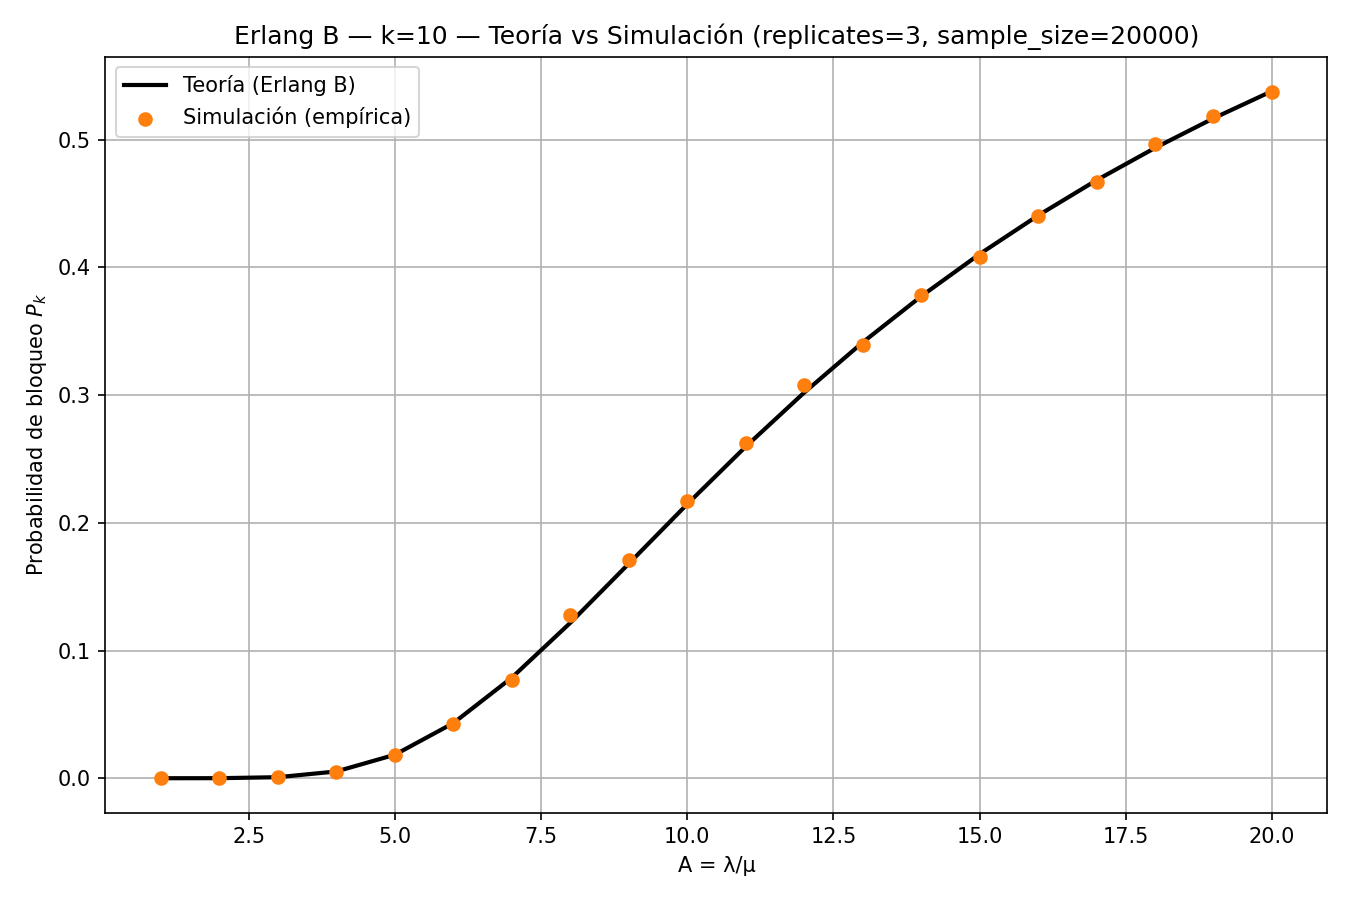
\includegraphics{plots/erlangb_validation_k10.png}
	\caption{Erlang B validation}
\end{figure}

\subsection{M\'etricas complementarias y Ley de Little}\label{muxe9tricas-complementarias-y-ley-de-little}

A continuaci\'on calculamos las m\'etricas relevantes para el sistema
M/M/k/k (Erlang B):

\begin{itemize}
	
	\bibitem{gross}
	      Tasa efectiva de llegadas:
	      \(\lambda_{\mathrm{eff}} = \lambda\, (1 - P_k)\) --- tasa de
	      transacciones que efectivamente entran al sistema.
	\bibitem{gross}
	      N\'umero medio de clientes en el sistema: \(L = \sum_{n=0}^k n\,P_n\).
	\bibitem{gross}
	      Tiempo medio en el sistema: \(W = 1/\mu\) (ya que \(W_q=0\)).
\end{itemize}

Verificaremos num\'ericamente la Ley de Little:
\(L = \lambda_{\mathrm{eff}}\cdot W\).

\subsection{Actividad 4 --- An\'alisis de sensibilidad y validaci\'on de resultados}\label{actividad-4-anuxe1lisis-de-sensibilidad-y-validaciuxf3n-de-resultados}

Esta secci\'on corresponde expl\'icitamente a la Actividad 4 de la
r\'ubrica. Se eval\'ua la sensibilidad del modelo M/M/k/k frente a
variaciones del tr\'afico ofrecido \(A=\lambda/\mu\), comparando resultados
de simulaci\'on (promedio y desviaci\'on est\'andar por r\'eplicas) contra la
soluci\'on te\'orica de Erlang B para la probabilidad de bloqueo \(P_k\).

Tambi\'en se contrasta el tiempo medio de espera te\'orico y simulado,
esperando \(W_q\approx0\) por la naturaleza sin cola del sistema M/M/k/k.
La concordancia entre ambas curvas confirma la consistencia
matem\'atica y la validez de implementaci\'on del motor de simulaci\'on.

\subsection{Actividad 5 --- Interpretaci\'on aplicada y decisiones de capacidad}\label{actividad-5-interpretaciuxf3n-aplicada-y-decisiones-de-capacidad}

Esta secci\'on cubre de forma expl\'icita la Actividad 5 de la r\'ubrica.
Con base en \(P_k\), \(\lambda_{\mathrm{eff}}\) y la Ley de Little, se
interpreta el impacto operacional sobre una pasarela de pagos: cuando
sube \(A\), aumenta el bloqueo y cae la tasa efectiva de transacciones
aceptadas. Esto permite definir reglas de escalamiento para dimensionar
\(k\) y mantener SLA de rechazo bajo umbrales de negocio.

\begin{tcolorbox}[breakable, size=fbox, boxrule=1pt, pad at break*=1mm,colback=cellbackground, colframe=cellborder]
	\prompt{In}{incolor}{ }{\boxspacing}
	\begin{lstlisting}
\PY{c+c1}{\PYZsh{} C\'alculo num\'erico de m\'etricas para M/M/k/k}
\PY{k+kn}{from}\PY{+w}{ }\PY{n+nn}{src}\PY{n+nn}{.}\PY{n+nn}{core}\PY{n+nn}{.}\PY{n+nn}{theory}\PY{+w}{ }\PY{k+kn}{import} \PY{n}{mmkk\PYZus{}stationary\PYZus{}probs}\PY{p}{,} \PY{n}{mmkk\PYZus{}mean\PYZus{}wait}

\PY{c+c1}{\PYZsh{} Par\'ametros de ejemplo (ajustables)}
\PY{n}{lam} \PY{o}{=} \PY{l+m+mf}{8.0}
\PY{n}{mu} \PY{o}{=} \PY{l+m+mf}{1.0}
\PY{n}{k} \PY{o}{=} \PY{l+m+mi}{10}
\PY{n}{A} \PY{o}{=} \PY{n}{lam} \PY{o}{/} \PY{n}{mu}

\PY{n}{Pn} \PY{o}{=} \PY{n}{mmkk\PYZus{}stationary\PYZus{}probs}\PY{p}{(}\PY{n}{lam}\PY{p}{,} \PY{n}{mu}\PY{p}{,} \PY{n}{k}\PY{p}{)}
\PY{n}{Pk} \PY{o}{=} \PY{n}{Pn}\PY{p}{[}\PY{o}{\PYZhy{}}\PY{l+m+mi}{1}\PY{p}{]}
\PY{n}{lambda\PYZus{}eff} \PY{o}{=} \PY{n}{lam} \PY{o}{*} \PY{p}{(}\PY{l+m+mf}{1.0} \PY{o}{\PYZhy{}} \PY{n}{Pk}\PY{p}{)}
\PY{n}{L} \PY{o}{=} \PY{n+nb}{sum}\PY{p}{(}\PY{n}{n} \PY{o}{*} \PY{n}{Pn}\PY{p}{[}\PY{n}{n}\PY{p}{]} \PY{k}{for} \PY{n}{n} \PY{o+ow}{in} \PY{n+nb}{range}\PY{p}{(}\PY{n+nb}{len}\PY{p}{(}\PY{n}{Pn}\PY{p}{)}\PY{p}{)}\PY{p}{)}
\PY{n}{W} \PY{o}{=} \PY{l+m+mf}{1.0} \PY{o}{/} \PY{n}{mu}  \PY{c+c1}{\PYZsh{} porque W\PYZus{}q = 0}

\PY{n+nb}{print}\PY{p}{(}\PY{l+s+sa}{f}\PY{l+s+s2}{\PYZdq{}}\PY{l+s+s2}{Parametros: lam=}\PY{l+s+si}{\PYZob{}}\PY{n}{lam}\PY{l+s+si}{\PYZcb{}}\PY{l+s+s2}{, mu=}\PY{l+s+si}{\PYZob{}}\PY{n}{mu}\PY{l+s+si}{\PYZcb{}}\PY{l+s+s2}{, k=}\PY{l+s+si}{\PYZob{}}\PY{n}{k}\PY{l+s+si}{\PYZcb{}}\PY{l+s+s2}{, A=}\PY{l+s+si}{\PYZob{}}\PY{n}{A}\PY{l+s+si}{\PYZcb{}}\PY{l+s+s2}{\PYZdq{}}\PY{p}{)}
\PY{n+nb}{print}\PY{p}{(}\PY{l+s+s2}{\PYZdq{}}\PY{l+s+s2}{P\PYZus{}n (n=0..k):}\PY{l+s+s2}{\PYZdq{}}\PY{p}{,} \PY{p}{[}\PY{n+nb}{round}\PY{p}{(}\PY{n}{p}\PY{p}{,} \PY{l+m+mi}{6}\PY{p}{)} \PY{k}{for} \PY{n}{p} \PY{o+ow}{in} \PY{n}{Pn}\PY{p}{]}\PY{p}{)}
\PY{n+nb}{print}\PY{p}{(}\PY{l+s+sa}{f}\PY{l+s+s2}{\PYZdq{}}\PY{l+s+s2}{P\PYZus{}k (probabilidad de bloqueo) = }\PY{l+s+si}{\PYZob{}}\PY{n}{Pk}\PY{l+s+si}{:}\PY{l+s+s2}{.6f}\PY{l+s+si}{\PYZcb{}}\PY{l+s+s2}{\PYZdq{}}\PY{p}{)}
\PY{n+nb}{print}\PY{p}{(}\PY{l+s+sa}{f}\PY{l+s+s2}{\PYZdq{}}\PY{l+s+s2}{Tasa efectiva lambda\PYZus{}eff = }\PY{l+s+si}{\PYZob{}}\PY{n}{lambda\PYZus{}eff}\PY{l+s+si}{:}\PY{l+s+s2}{.6f}\PY{l+s+si}{\PYZcb{}}\PY{l+s+s2}{\PYZdq{}}\PY{p}{)}
\PY{n+nb}{print}\PY{p}{(}\PY{l+s+sa}{f}\PY{l+s+s2}{\PYZdq{}}\PY{l+s+s2}{Numero medio en sistema L = }\PY{l+s+si}{\PYZob{}}\PY{n}{L}\PY{l+s+si}{:}\PY{l+s+s2}{.6f}\PY{l+s+si}{\PYZcb{}}\PY{l+s+s2}{\PYZdq{}}\PY{p}{)}
\PY{n+nb}{print}\PY{p}{(}\PY{l+s+sa}{f}\PY{l+s+s2}{\PYZdq{}}\PY{l+s+s2}{Tiempo medio en sistema W = }\PY{l+s+si}{\PYZob{}}\PY{n}{W}\PY{l+s+si}{:}\PY{l+s+s2}{.6f}\PY{l+s+si}{\PYZcb{}}\PY{l+s+s2}{\PYZdq{}}\PY{p}{)}
\PY{n+nb}{print}\PY{p}{(}\PY{l+s+s2}{\PYZdq{}}\PY{l+s+s2}{Verificaci\'on Ley de Little: L vs lambda\PYZus{}eff * W =\PYZgt{}}\PY{l+s+s2}{\PYZdq{}}\PY{p}{,} \PY{n}{L}\PY{p}{,} \PY{n}{lambda\PYZus{}eff} \PY{o}{*} \PY{n}{W}\PY{p}{)}
\PY{n+nb}{print}\PY{p}{(}\PY{l+s+s2}{\PYZdq{}}\PY{l+s+s2}{Diferencia absoluta:}\PY{l+s+s2}{\PYZdq{}}\PY{p}{,} \PY{n+nb}{abs}\PY{p}{(}\PY{n}{L} \PY{o}{\PYZhy{}} \PY{n}{lambda\PYZus{}eff} \PY{o}{*} \PY{n}{W}\PY{p}{)}\PY{p}{)}
\PY{n+nb}{print}\PY{p}{(}\PY{l+s+s2}{\PYZdq{}}\PY{l+s+s2}{Error relativo:}\PY{l+s+s2}{\PYZdq{}}\PY{p}{,} \PY{n+nb}{abs}\PY{p}{(}\PY{n}{L} \PY{o}{\PYZhy{}} \PY{n}{lambda\PYZus{}eff} \PY{o}{*} \PY{n}{W}\PY{p}{)} \PY{o}{/} \PY{p}{(}\PY{n}{L} \PY{k}{if} \PY{n}{L}\PY{o}{\PYZgt{}}\PY{l+m+mi}{0} \PY{k}{else} \PY{l+m+mf}{1.0}\PY{p}{)}\PY{p}{)}
\end{lstlisting}
\end{tcolorbox}

\subsection{Conclusi\'on: Aplicaci\'on a Pasarelas de Pago}\label{conclusiuxf3n-aplicaciuxf3n-a-pasarelas-de-pago}

En el contexto de una pasarela de pagos bancarios, cada ``cliente'' en
el modelo representa una petici\'on de transacci\'on entrante, y cada uno de
los \(k\) servidores modela una instancia de servicio (microservicio)
capaz de procesar transacciones en paralelo. La probabilidad de bloqueo
\(P_k\) cuantifica la fracci\'on de transacciones rechazadas
inmediatamente por falta de capacidad --- es decir, cuando las \(k\)
instancias est\'an ocupadas.

La tasa de tr\'afico ofrecido \(A=\lambda/\mu\) es cr\'itica: al incrementar
\(A\) (m\'as solicitudes por unidad de tiempo, o menor capacidad de
procesamiento por servidor), \(P_k\) crece r\'apidamente y la tasa
efectiva de aceptaci\'on \(\lambda_{\mathrm{eff}}=\lambda(1-P_k)\)
disminuye. Monitorear \(A\) y \(P_k\) permite dimensionar la
infraestructura (escalar horizontalmente el n\'umero de servidores \(k\) o
mejorar la tasa de servicio \(\mu\)) para mantener el nivel de rechazo
por debajo de un umbral aceptable. En producci\'on esto se traduce en
alertas APM y reglas de escalado autom\'atico basadas en m\'etricas de
bloqueo y tr\'afico.


\section{Conclusiones y Trabajos Futuros}
El análisis del modelo M/M/k/k (Erlang B) ha demostrado la relevancia de comprender los sistemas sin cola frente a la limitación de recursos.
\textbf{Conclusiones principales:} La probabilidad de bloqueo crece exponencialmente con la carga ofrecida $A$, afectando la tasa efectiva de servicio. Las simulaciones confirman la exactitud teórica cuando las llegadas son verdaderamente de Poisson.
\textbf{Aplicaciones reales:} Este modelo es aplicable al dimensionamiento de microservicios, pasarelas de pago y asignación de canales de radio, donde no hay encolamiento \cite{itu}.
\textbf{Trabajos futuros:} Como trabajo futuro se propone evaluar modelos con encolamiento finito (M/M/k/c) \cite{kleinrock} o considerar distribuciones de tiempo de servicio de cola pesada para acercar el modelo aún más al tráfico empírico de redes LAN, como el observado en los datasets de Bellcore.


\section{Referencias}
\begin{thebibliography}{9}
\bibitem{gross} Gross, D., Shortle, J. F., Thompson, J. M., \& Harris, C. M. (2018). \textit{Fundamentals of Queueing Theory} (5th ed.). Wiley.
\bibitem{cooper} Cooper, R. B. (1981). \textit{Introduction to Queueing Theory} (2nd ed.). North Holland.
\bibitem{kleinrock} Kleinrock, L. (1975). \textit{Queueing Systems, Volume 1: Theory}. Wiley.
\bibitem{ross} Ross, S. M. (2019). \textit{Introduction to Probability Models} (12th ed.). Academic Press.
\bibitem{itu} ITU-T Recommendation E.600 (1993). \textit{Terms and definitions of traffic engineering}.
\end{thebibliography}

\end{document}
